% Kompilacja z katalogu projektu:
% latexmk -pdf -interaction=nonstopmode -halt-on-error -outdir=tmp/latex docs/presentation.tex
% Następnie: cp tmp/latex/presentation.pdf presentation.pdf
% Notatki prowadzącego są zapisane w poleceniach \note i domyślnie ukryte.
% Aby je wyświetlić, zmień hide notes na show notes w ustawieniu poniżej.
% Prezentacja utrwala zapisane wyniki z 16.11.2026, bez oczekiwania na nowe treningi.
\documentclass[12pt,aspectratio=169]{beamer}
\usepackage[T1]{fontenc}
\usepackage[utf8]{inputenc}
\usepackage[polish]{babel}
\usepackage{lmodern}
\usepackage{tgheros}
\usepackage{amsmath,booktabs,array,tabularx}
\usepackage{graphicx}
\usepackage{pgfplots}
\usetikzlibrary{arrows.meta}
\pgfplotsset{compat=1.18}
\usepackage{appendixnumberbeamer}

\definecolor{Ink}{HTML}{152B39}
\definecolor{Muted}{HTML}{536672}
\definecolor{Teal}{HTML}{007F78}
\definecolor{Coral}{HTML}{C9553F}
\definecolor{Mist}{HTML}{DCE4E8}
\definecolor{Paper}{HTML}{FAFBFC}
\definecolor{Blue}{HTML}{496FA4}
\setbeamercolor{normal text}{fg=Ink,bg=Paper}
\setbeamercolor{frametitle}{fg=Ink,bg=Paper}
\setbeamercolor{structure}{fg=Teal}
\setbeamercolor{alerted text}{fg=Teal}
\setbeamercolor{footline}{fg=Muted,bg=Paper}
\setbeamerfont{frametitle}{size=\Large,series=\bfseries}
\setbeamerfont{footline}{size=\scriptsize}
\setbeamersize{text margin left=9mm,text margin right=9mm}
\setbeamertemplate{navigation symbols}{}
\setbeamertemplate{itemize item}{\small\textbullet}
\setbeamertemplate{itemize subitem}{\small\textbullet}
\setbeamertemplate{frametitle}{\vspace{3.5mm}\insertframetitle\par\vspace{2mm}}
\newcommand{\footerlabel}{Pong / Q-learning}
\setbeamertemplate{footline}{%
  \begin{beamercolorbox}[wd=\paperwidth,ht=3mm,dp=3mm,leftskip=9mm,rightskip=9mm]{footline}%
    \usebeamerfont{footline}\hfill\insertframenumber
  \end{beamercolorbox}}
\setbeameroption{hide notes}
\graphicspath{{docs/figures/}{figures/}}
\renewcommand{\tabularxcolumn}[1]{>{\raggedright\arraybackslash}p{#1}}
\newcolumntype{L}[1]{>{\raggedright\arraybackslash}p{#1}}
\renewcommand{\arraystretch}{1.28}
\newcommand{\smalltext}[1]{\par{\small\color{Muted}#1\par}}
\newcommand{\source}[1]{\par\vfill{\fontsize{8.5}{10}\selectfont\color{Muted}#1\par}}
\newcommand{\takeaway}[1]{\par\vspace{2mm}{\color{Teal}\bfseries #1\par}}
\newcommand{\bigvalue}[1]{{\fontsize{34}{37}\selectfont\bfseries\color{Teal}#1}}
\newcommand{\resultlegend}{%
  {\small\textcolor{Teal}{\rule{3mm}{2mm}} Wygrana\qquad
  \textcolor{Coral}{\rule{3mm}{2mm}} Porażka\qquad
  \textcolor{Muted}{\rule{3mm}{2mm}} Limit 20 s}}
\pgfplotsset{deck/.style={
  axis line style={draw=Mist},tick style={draw=none},
  tick label style={font=\small,color=Muted},
  label style={font=\small,color=Muted},
  grid style={draw=Mist},
  axis on top,clip=false,
  /pgf/number format/use comma,
  /pgf/number format/1000 sep={\,}
}}

\title{Pong: przeciwnik uczący się grać}
\author{Artur Zamorowski \and Kacper Wojtowicz \and Rafał Wybraniec}
\date{16 listopada 2026}
\hypersetup{pdftitle={Pong: przeciwnik uczący się grać},
pdfauthor={Artur Zamorowski, Kacper Wojtowicz, Rafał Wybraniec},pdflang={pl-PL}}

\begin{document}
\begin{frame}[plain]\relax
{\fontsize{42}{46}\selectfont\bfseries Pong\par}
\vspace{4mm}
{\LARGE Uczenie agenta metodą Q-learningu\par}
\vfill
\smalltext{Artur Zamorowski, Kacper Wojtowicz, Rafał Wybraniec}
\smalltext{16 listopada 2026}
\note{Celem było przygotowanie przeciwnika, który sam uczy się sterować paletką.
Opowiemy, jak pojedyncze decyzje zamieniają się w wyuczoną strategię, co dał
pierwszy eksperyment i jak wypadła kolejna wersja. Około 12--15 minut.
Podstawą jest sprawozdanie, a drugi etap uzupełniają zapisane wyniki projektu.}
\end{frame}

\begin{frame}{Nasza wersja Ponga}\relax


\begin{columns}[c,onlytextwidth]
\column{0.59\textwidth}
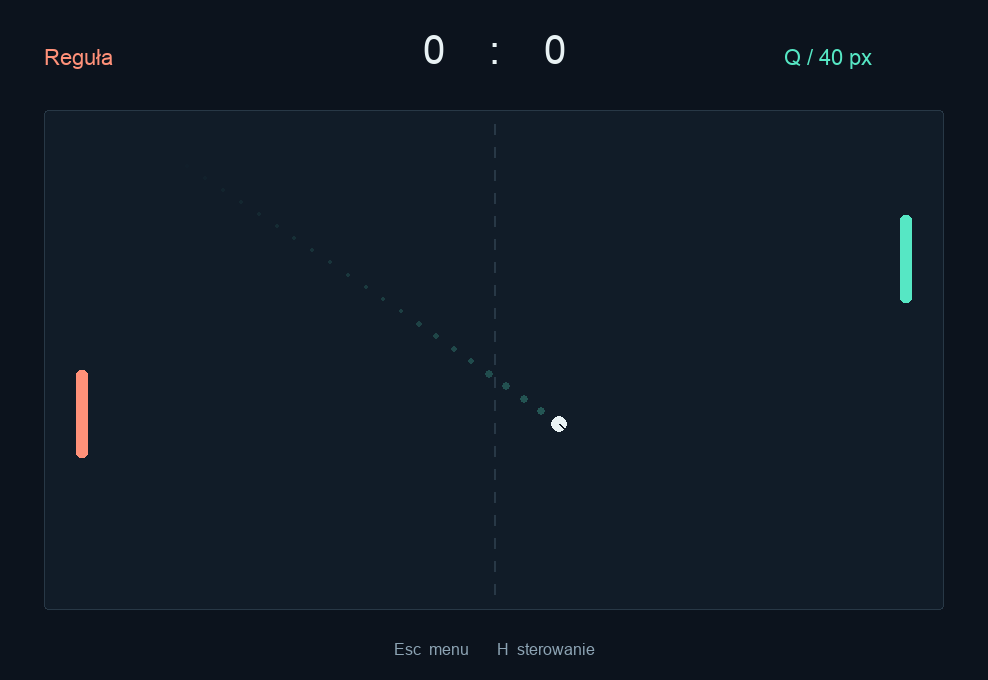
\includegraphics[width=\linewidth,height=5.4cm,keepaspectratio]{game.png}
\column{0.37\textwidth}
Nasz agent steruje prawą paletką. Po lewej gra Tracker, który przesuwa paletkę w stronę piłki.
\par\vspace{5mm}
Obaj gracze mają te same ograniczenia ruchu.
\end{columns}

\note{Na ekranie jest widok pierwszego modelu z siatką 40 px.
Tracker ma stałą regułę i nie uczy się. Agent podejmuje decyzje na podstawie
tablicy Q. Mecz w interfejsie trwa do siedmiu punktów. W treningu jednostką
doświadczenia jest jedna wymiana. Źródło: docs/report.tex, Gra i symulacja.

Fizyka pracuje z krokiem 1/120 s, a decyzja zapada co cztery kroki.
Paletka nie przeskakuje na docelową wysokość. Blisko środka paletki odbicie
jest bardziej poziome, przy końcu bardziej strome. Rotacja występuje
w fizyce obu etapów, lecz pierwszy agent nie ma jej w obserwacji.
Źródło: docs/report.tex, Gra i symulacja, oraz src/pong/physics.py.

Agent steruje prawą paletką. Tracker po lewej śledzi bieżącą wysokość piłki. Obaj mają te same ograniczenia ruchu. Zrzut przedstawia pierwszy model, W32.}
\end{frame}

\begin{frame}{Jak agent wybiera ruch}\relax


Dla każdej sytuacji tablica Q przechowuje oceny trzech ruchów.
\par\vspace{5mm}
\begin{center}
{\large
\begin{tabular}{@{}lccc@{}}
\toprule
& W górę & Postój & W dół\\
\midrule
$Q(s,a)$ & $0{,}12$ & $0{,}08$ & \textcolor{Teal}{$\boldsymbol{0{,}31}$}\\
\bottomrule
\end{tabular}}
\end{center}
\vspace{5mm}
W tym przykładzie agent wybierze ruch w dół, bo ma on najwyższą ocenę.
\source{Liczby służą do objaśnienia działania tablicy.}

\note{Agent otrzymuje liczby z symulatora, a nie obraz ekranu. Nie obserwuje
paletki przeciwnika. Dyskretyzacja pozwala korzystać ze skończonej tablicy.
W pierwszym etapie kodujemy sześć wielkości. Dwie sytuacje przypisane do
jednego stanu muszą korzystać z tych samych ocen akcji.
Źródło: docs/report.tex, Obserwacja, stan i akcje.

Wartość Q nie jest procentowym prawdopodobieństwem wygranej.
To ocena sumy przyszłych nagród, z mniejszą wagą tych bardziej odległych.
Losowe ruchy w treningu to eksploracja epsilon-greedy. W pierwszym
eksperymencie epsilon maleje z 0,9 do 0,02 przez 50 tys. wymian.
W aktualnej konfiguracji drugiego etapu: z 0,7 do 0,02 przez 100 tys.
Na starcie Q jest zerowe. Źródło: docs/report.tex i config.yaml.

W modelu siatkowym położenia dzielimy na przedziały. Wysokości 310 i 319 px należą do tego samego przedziału 40 px. Q oznacza ocenę przyszłych nagród. W treningu agent także eksploruje, a podczas oceny wybiera najlepszą znaną akcję.}
\end{frame}

\begin{frame}{Za co agent dostaje nagrodę}\relax


\begin{columns}[T,onlytextwidth]
\column{0.30\textwidth}\bigvalue{$+1$}\par\vspace{3mm}za zdobycie punktu
\column{0.30\textwidth}{\color{Coral}\fontsize{34}{37}\selectfont $-1$}\par\vspace{3mm}za stratę punktu
\column{0.30\textwidth}\bigvalue{$+0{,}2$}\par\vspace{3mm}za odbicie piłki
\end{columns}
\vspace{12mm}
Po każdym ruchu agent aktualizuje jego ocenę w tablicy Q na podstawie nagrody i nowej sytuacji na boisku.

\note{Po każdym ruchu zmienia się jedna komórka Q. Agent porównuje wcześniejszą
ocenę z otrzymaną nagrodą i oceną następnego stanu. Tak informacja o dobrych
skutkach dociera także do wcześniejszych decyzji. W pierwszym eksperymencie
porównaliśmy nagrodę 0 i +0,2 za odbicie. Finaliści i nowy model używają +0,2.
Przerwanie po 20 s nie zeruje przyszłej wartości w aktualizacji, bo nie jest
naturalnym zakończeniem punktu. Źródło: docs/report.tex, Nagrody i aktualizacja.

Pełny wzór aktualizacji znajduje się na slajdzie dodatkowym. Nagrodę za odbicie porównaliśmy z brakiem takiej nagrody. Pokazane +0,2 stosują finaliści i nowy agent.}
\end{frame}

\begin{frame}{Pierwszy eksperyment}\relax


Sprawdziliśmy 48 zestawów parametrów. Najlepsze trenowaliśmy dłużej.
\par\vspace{4mm}
\begin{center}
\begin{tabular}{@{}cc@{}}
\toprule
Liczba wariantów & Trening do\\
\midrule
48 & 50 tys. epizodów\\
8 & 200 tys. epizodów\\
3 & 500 tys. epizodów\\
\bottomrule
\end{tabular}
\end{center}
\vspace{3mm}
Każdego finalistę trenowaliśmy trzykrotnie, z różnymi ziarnami losowania.

\note{Ziarno ustala przebieg losowania. Różne ziarna dają niezależne przebiegi
treningu tego samego wariantu. Łącznie wykonaliśmy 7,5 mln epizodów.
Pierwszy odsiew odbywał się na jednym ziarnie, więc mógł odrzucić ustawienia,
które potrzebowałyby więcej czasu. Wariant W32 wybraliśmy na dodatkowych
2000 serwisach. Źródło: docs/report.tex, Przeszukiwanie parametrów.

W32: komórka 40, alfa 0,12, gamma 0,98. W42: komórka 50,
alfa 0,03, gamma 0,999. W36: komórka 40, alfa 0,12, gamma 0,999.
Wszyscy finaliści mają nagrodę za odbicie +0,2. Znak plus/minus opisuje
odchylenie standardowe, nie przedział ufności.

W finale trzy ziarna na wariant: 7, 23 i 41. Komórki: 20, 25, 40 i 50 px. Alfa: 0,03 i 0,12. Gamma: 0,98; 0,995; 0,999. Nagroda za odbicie: 0 i +0,2. Końcowe średnie wygranych: W32 26,6 procent, W42 26,5 procent, W36 24,4 procent. Pełne wyniki i parametry: docs/report.tex.}
\end{frame}

\begin{frame}{Przebieg uczenia W32}\relax

\begin{center}
\begin{tikzpicture}
\begin{axis}[deck,width=12cm,height=4.7cm,
  xmin=0,xmax=530,ymin=0,ymax=35,
  xtick={0,100,200,350,500},ytick={0,10,20,30},ymajorgrids,
  xlabel={Epizody [tys.]},ylabel={Wygrane [\%]}]
\addplot[Teal,very thick,mark=*] coordinates {(25,6.5)(50,15.5)(100,21)(200,23.25)(350,16.25)(500,25.75)};
\end{axis}
\end{tikzpicture}
\end{center}
Dalszy trening czasem pogarszał wynik, dlatego zachowywaliśmy najlepszą tablicę.
\source{Jeden trening W32. Każdy pomiar obejmował 400 wymian z Trackerem.}

\note{To nie są wyniki końcowego testu ani średnie z trzech ziaren.
Pokazujemy jeden przebieg W32 z ziarnem 7, aby wyjaśnić sens zapisywania
najlepszej tablicy w trakcie treningu.
Zmiany oceny mogą wynikać ze zmian polityki oraz z ograniczonego zestawu
walidacyjnego. Slajd pokazuje zmiany umiejętności jednego agenta
podczas treningu.

Zachowujemy najlepszy checkpoint. W32: 23,25 procent po 200 tys. epizodów i 16,25 procent po 350 tys. Źródło: historyczne grid\_training.csv, zachowane w docs/data/experiments.zip.}
\end{frame}

\begin{frame}{Wyniki pierwszego eksperymentu}\relax

\begin{center}
\resultlegend\par\vspace{4mm}
\begin{tikzpicture}
\begin{axis}[deck,xbar stacked,width=11.7cm,height=3.9cm,
  xmin=0,xmax=100,ymin=-0.5,ymax=1.5,bar width=9mm,
  ytick={0,1},yticklabels={W32,Model początkowy},
  xtick={0,25,50,75,100},xlabel={Udział wymian [\%]},
  nodes near coords,nodes near coords style={font=\small,text=white},
  every node near coord/.append style={/pgf/number format/fixed,/pgf/number format/precision=2,/pgf/number format/fixed zerofill}]
\addplot[fill=Teal,draw=none] coordinates {(28.64,0)(15.16,1)};
\addplot[fill=Coral,draw=none] coordinates {(48.24,0)(76.10,1)};
\addplot[fill=Muted,draw=none] coordinates {(23.12,0)(8.74,1)};
\end{axis}
\end{tikzpicture}
\end{center}
W32 wygrywał częściej niż model początkowy, ale nadal przegrywał prawie połowę wymian.
\source{Test obejmował 5000 wspólnych serwisów. Pokazujemy W32 z ziarnem 7.}

\note{W32 ma komórkę 40 px, alfa 0,12, gamma 0,98, nagrodę za odbicie +0,2
i checkpoint po 500 tys. epizodów. Model początkowy trenowano 50 tys.
W32 wygrał 1432 i przegrał 2412 prób, a 1156 osiągnęło limit czasu.
Sama poprawa odsetka wygranych nie oznacza pokonania przeciwnika.

Źródło: docs/report.tex, Wyniki modelu bazowego. Pierwotne CSV zachowano w docs/data/experiments.zip.}
\end{frame}

\begin{frame}{Siatka położenia piłki}\relax

\begin{columns}[T,onlytextwidth]
\column{0.48\textwidth}
\centering Baseline W32\par
\smalltext{Równe komórki $40\times40$ px}
\vspace{2mm}
\begin{tikzpicture}[x=0.006cm,y=-0.006cm,font=\small]
  \path[use as bounding box] (-80,-40) rectangle (930,540);
  \foreach \x in {0,40,...,880} \draw[Mist] (\x,0) -- (\x,500);
  \foreach \y in {0,40,...,480} \draw[Mist] (0,\y) -- (900,\y);
  \fill[Teal,fill opacity=0.23] (760,200) rectangle (800,240);
  \draw[Muted] (0,0) rectangle (900,500);
  \fill[Teal] (780,205) circle (8);
  \fill[Ink] (856,176) rectangle (868,264);
  \node[anchor=east,text=Muted] at (-18,0) {0};
  \node[anchor=east,text=Muted] at (-18,500) {500};
  \node[anchor=north,text=Muted] at (0,520) {0};
  \node[anchor=north,text=Muted] at (450,520) {450};
  \node[anchor=north,text=Muted] at (900,520) {900};
\end{tikzpicture}
\par\vspace{1.5mm}
Piłka: kolumna i wiersz.\par
Paletka: osobny wiersz co 40 px.
\column{0.48\textwidth}
\centering Ulepszony model\par
\smalltext{8 kolumn, wysokość co 25 px}
\vspace{2mm}
\begin{tikzpicture}[x=0.006cm,y=-0.006cm,font=\small]
  \path[use as bounding box] (-80,-40) rectangle (930,540);
  \foreach \x in {0,450,600,700,760,800,825,840,900}
    \draw[Mist] (\x,0) -- (\x,250);
  \foreach \y in {0,25,...,250} \draw[Mist] (0,\y) -- (900,\y);
  \fill[Teal,fill opacity=0.23] (760,200) rectangle (800,225);
  \draw[Muted] (0,0) rectangle (900,500);
  \draw[Muted,dashed] (0,250) -- (900,250);
  \fill[Teal] (780,205) circle (8);
  \fill[Ink] (856,176) rectangle (868,264);
  \draw[Muted,-{Latex[length=2mm]}] (450,420) -- (450,305);
  \node[text=Muted] at (450,460) {odbicie do góry};
  \node[anchor=east,text=Muted] at (-18,0) {0};
  \node[anchor=east,text=Muted] at (-18,250) {250};
  \node[anchor=east,text=Muted] at (-18,500) {500};
  \node[anchor=north,text=Muted] at (0,520) {0};
  \node[anchor=north,text=Muted] at (450,520) {450};
  \node[anchor=north,text=Muted] at (900,520) {900};
\end{tikzpicture}
\par\vspace{1.5mm}
Piłka: siatka z symetrią góra--dół.\par
Paletka: 20 przedziałów $y_b-y_p$.
\smalltext{Blisko zera co 10 px.}
\end{columns}

\note{Agent otrzymuje liczby z symulatora. Współrzędne oznaczają środki
piłki i własnej, prawej paletki. Pozycja pozioma paletki jest stała,
więc w obserwacji występuje tylko jej wysokość i prędkość pionowa.
Baseline kodował osobno wiersz piłki i wiersz paletki. W nowym stanie
wiersz paletki zastępujemy różnicą dokładnych współrzędnych yb-yp,
obliczoną przed podziałem na przedziały. Zachowujemy wysokość piłki,
bo ma znaczenie dla odbić od górnej i dolnej ściany.

Progi x wynoszą 450, 600, 700, 760, 800, 825 i 840 px.
Przedziały błędu blisko zera mają szerokość 10 px, dalej są szersze.
Nowe kodowanie dodatkowo odbija dolne sytuacje do górnej połowy,
co wyjaśniają kolejne slajdy. Stan opisuje bieżącą sytuację,
bez przewidywanego miejsca uderzenia piłki.

Dodaliśmy rotację i dokładniejszy opis prędkości. Budżet wzrósł
z 500 tys. do 2 mln epizodów. Alfa zmieniła się z 0,12 na 0,15,
a gamma z 0,98 na 0,995. Wybrany checkpoint pochodzi z 1,8 mln epizodów.
Sześć konfiguracji trenowano do 2 mln epizodów, a wybrany wariant
powtórzono z trzema ziarnami. Nie przypisujemy całej poprawy samemu
kodowaniu pozycji.
Źródła: docs/report.tex, Usprawnienie modelu, src/pong/agents.py,
src/pong/physics.py i config.yaml.}
\end{frame}

\begin{frame}{Co gubiła siatka 40 px}\relax

Zbliżenie na wiersz od 200 do 240 px. Współrzędna $y$ rośnie w dół.
\par\vspace{3mm}
\begin{columns}[T,onlytextwidth]
\column{0.48\textwidth}
\centering Sytuacja A\par\vspace{1mm}
\begin{tikzpicture}[x=1cm,y=1cm,font=\small]
  \path[use as bounding box] (-0.6,-0.05) rectangle (5.3,2.85);
  \fill[Teal,fill opacity=0.12] (0,0.75) rectangle (5.1,1.75);
  \foreach \y/\label in {2.75/160,1.75/200,0.75/240}
    {\draw[Mist] (0,\y) -- (5.1,\y);
     \node[anchor=east,text=Muted] at (-0.1,\y) {\label};}
  \fill[Teal] (1.6,1.625) circle (0.075);
  \node[anchor=south,text=Ink] at (1.6,1.79) {piłka: 205};
  \fill[Ink] (4.8,0.15) rectangle (4.9,2.35);
  \draw[Ink] (4.65,1.25) -- (5.05,1.25);
  \node[anchor=east,text=Ink] at (4.55,1.25) {środek: 220};
\end{tikzpicture}
\par\vspace{2mm}
Baseline: wiersze $(5,5)$.\par
\textcolor{Teal}{Nowy model: $205-220=-15$ px.}\par
\smalltext{Piłka nad środkiem paletki.}
\column{0.48\textwidth}
\centering Sytuacja B\par\vspace{1mm}
\begin{tikzpicture}[x=1cm,y=1cm,font=\small]
  \path[use as bounding box] (-0.6,-0.05) rectangle (5.3,2.85);
  \fill[Teal,fill opacity=0.12] (0,0.75) rectangle (5.1,1.75);
  \foreach \y/\label in {2.75/160,1.75/200,0.75/240}
    {\draw[Mist] (0,\y) -- (5.1,\y);
     \node[anchor=east,text=Muted] at (-0.1,\y) {\label};}
  \fill[Teal] (1.6,1.25) circle (0.075);
  \node[anchor=north,text=Ink] at (1.6,1.09) {piłka: 220};
  \fill[Ink] (4.8,0.525) rectangle (4.9,2.725);
  \draw[Ink] (4.65,1.625) -- (5.05,1.625);
  \node[anchor=east,text=Ink] at (4.55,1.625) {środek: 205};
\end{tikzpicture}
\par\vspace{2mm}
Baseline: wiersze $(5,5)$.\par
\textcolor{Teal}{Nowy model: $220-205=+15$ px.}\par
\smalltext{Piłka pod środkiem paletki.}
\end{columns}

\note{Przykłady są objaśniające. Przyjmujemy identyczne x i pozostałe
składniki obserwacji. W baseline dzielenie przez 40 i zaokrąglenie
w dół daje 5 dla 205 oraz dla 220. Obie pary trafiają do tego samego
wiersza tablicy Q, choć piłka jest raz nad środkiem paletki, a raz pod nim.
Obie wysokości piłki należą również do tego samego nowego przedziału
co 25 px, od 200 do 225. To sam składnik różnicy wysokości rozróżnia
tu sytuacje: -15 trafia do przedziału od -20 do -10,
a +15 do przedziału od 10 do 20 px.

Obie piłki są w górnej połowie boiska, więc przykład nie wymaga
odwracania współrzędnych. Ujemna różnica oznacza piłkę nad środkiem,
dodatnia pod środkiem. Sama różnica nie narzuca ruchu: agent uwzględnia
także prędkości, spin i położenie poziome. To bieżące ustawienie,
nie przewidywane miejsce przyszłego uderzenia.
Źródło kodowania: src/pong/agents.py, metoda state.}
\end{frame}

\begin{frame}{Symetria góra--dół}\relax

Te ustawienia są lustrzanymi odbiciami na boisku 500 px.
\par\vspace{3mm}
\begin{columns}[T,onlytextwidth]
\column{0.48\textwidth}
\centering Górna sytuacja\par\vspace{2mm}
\begin{tikzpicture}[x=1cm,y=1cm,font=\small]
  \path[use as bounding box] (-0.55,-0.15) rectangle (5.4,2.75);
  \draw[Mist] (0,0) rectangle (5.1,2.5);
  \draw[Mist,dashed] (0,1.25) -- (5.1,1.25);
  \node[anchor=east,text=Muted] at (-0.12,2.5) {0};
  \node[anchor=east,text=Muted] at (-0.12,1.25) {250};
  \node[anchor=east,text=Muted] at (-0.12,0) {500};
  \fill[Teal] (2.25,2) circle (0.065);
  \node[anchor=south,text=Ink] at (2.25,2.12) {piłka: 100};
  \fill[Ink] (4.75,1.28) rectangle (4.81,1.72);
  \node[anchor=east,text=Ink] at (4.57,1.5) {paletka: 200};
\end{tikzpicture}
\column{0.48\textwidth}
\centering Dolna sytuacja\par\vspace{2mm}
\begin{tikzpicture}[x=1cm,y=1cm,font=\small]
  \path[use as bounding box] (-0.55,-0.15) rectangle (5.4,2.75);
  \draw[Mist] (0,0) rectangle (5.1,2.5);
  \draw[Mist,dashed] (0,1.25) -- (5.1,1.25);
  \node[anchor=east,text=Muted] at (-0.12,2.5) {0};
  \node[anchor=east,text=Muted] at (-0.12,1.25) {250};
  \node[anchor=east,text=Muted] at (-0.12,0) {500};
  \fill[Teal] (2.25,0.5) circle (0.065);
  \node[anchor=north,text=Ink] at (2.25,0.38) {piłka: 400};
  \fill[Ink] (4.75,0.78) rectangle (4.81,1.22);
  \node[anchor=east,text=Ink] at (4.57,1) {paletka: 300};
\end{tikzpicture}
\end{columns}
\par\vspace{1mm}
Dolną sytuację odbijamy przed odczytem Q: $y'=500-y$.
\par\vspace{2mm}
{\centering $y_b'=500-400=100,\qquad y_p'=500-300=200$\par}
\vspace{2mm}
Lustrzane sytuacje korzystają z tego samego wiersza tablicy Q.

\note{Rysunki pokazują pozycje w pikselach. Oś y rośnie w dół,
a linia przerywana oznacza poziomą oś boiska na wysokości 250 px.
To odbicie góra--dół: x piłki pozostaje bez zmian, agent nadal
steruje prawą paletką. Nie zamieniamy graczy stronami.
Warunek w kodzie sprawdza wysokość piłki. Gdy yb przekracza H/2,
przekształcamy zarówno yb, jak i yp przez H-y.
Górny przykład ma różnicę 100-200=-100. Dolny przed odbiciem ma
400-300=+100, a po odbiciu ponownie 100-200=-100.

Wspólny stan wymaga także lustrzanych prędkości pionowych i rotacji,
oraz jednakowych x i vx. Ich znaki i mapowanie akcji pokazuje
następny slajd. W baseline oba ustawienia miały osobne wiersze Q.
Nowy model współdzieli doświadczenie między takimi sytuacjami.

Liczba wierszy W32 wynosi 23 razy 13 razy 13 razy 18 = 69 966.
Nowe kodowanie ma 8 razy 10 razy 20 razy 4 razy 7 razy 5 razy 5
= 1 120 000 wierszy. Symetria zmniejsza nową tablicę względem
analogicznego kodowania bez symetrii, a nie względem baseline.
Źródła: src/pong/agents.py, state, oraz docs/report.tex,
Stan względny, rotacja i symetria.}
\end{frame}

\begin{frame}{Symetria przy wyborze ruchu}\relax

\begin{center}
\begin{tikzpicture}[x=1cm,y=1cm]
  \path[use as bounding box] (0,-0.25) rectangle (13.8,3.8);
  \node[text=Ink] at (6.9,3.5) {Wspólny wiersz Q wybiera np. ruch w górę};
  \draw[Muted,-{Latex[length=2mm]}] (6.5,3.1) -- (6.5,2.8) -- (3,2.8) -- (3,2.4);
  \draw[Muted,-{Latex[length=2mm]}] (7.3,3.1) -- (7.3,2.8) -- (10.8,2.8) -- (10.8,2.4);
  \node[text=Ink] at (3,2.1) {Górna sytuacja};
  \node[text=Ink] at (10.8,2.1) {Dolna sytuacja};
  \fill[Ink] (2.65,0.65) rectangle (2.76,1.55);
  \fill[Ink] (10.45,0.65) rectangle (10.56,1.55);
  \draw[Teal,very thick,-{Latex[length=3mm]}] (3.3,0.65) -- (3.3,1.55);
  \draw[Teal,very thick,-{Latex[length=3mm]}] (11.1,1.55) -- (11.1,0.65);
  \node[text=Ink] at (3,0.2) {Wykonujemy ruch w górę};
  \node[text=Ink] at (10.8,0.2) {Wykonujemy ruch w dół};
\end{tikzpicture}
\end{center}
Postój pozostaje postojem. Ruch w dół zamieniamy analogicznie.
\par\vspace{3mm}
Przy odbiciu stanu odwracamy też pionowe prędkości i spin.
Położenie $x$ i prędkość pozioma pozostają takie same.

\note{Przykładowo, jeżeli wspólny wiersz Q najwyżej ocenia ruch w górę,
to w górnej sytuacji wykonujemy ruch w górę, a w jej dolnym odbiciu
ruch w dół. Postój pozostaje postojem. To ilustracja mapowania,
nie deklaracja konkretnej akcji wytrenowanego modelu.

Dla dolnej sytuacji stan zmienia znaki vy, prędkości paletki pvy
i spinu. Na przykład vy=-180 w dolnej sytuacji kodujemy jako +180
w górnej. Dzięki temu model opisuje fizycznie lustrzany ruch.
Poziome x i vx zachowujemy. Funkcja orientation zwraca -1 dla
piłki w dolnej połowie i +1 dla pozostałych sytuacji.
Action mnoży kierunek z tablicy Q przez tę orientację.
Update stosuje to samo odwrócenie do wykonanej akcji, aby nagroda
trafiła do odpowiedniej komórki we wspólnym wierszu Q.

Dlatego odbicie w dolnej połowie uczy też odpowiadającego mu
zachowania w górnej. Nie trzeba osobno zbierać obu doświadczeń.
Źródło: src/pong/agents.py, metody state, orientation, action i update.}
\end{frame}

\begin{frame}{Pozostałe zmiany}\relax

{\large
Dodaliśmy rotację piłki i dokładniejsze przedziały prędkości.
\par\vspace{7mm}
Zwiększyliśmy budżet treningu z 500 tys. do 2 mln epizodów
i zmieniliśmy parametry uczenia.
\par}

\note{Ten slajd zachowuje pozostałe zmiany omawiane przed rozwinięciem
wyjaśnienia reprezentacji. Alfa wzrosła z 0,12 do 0,15, gamma z 0,98
do 0,995. Wybrany model pochodzi z checkpointu po 1,8 mln epizodów.
Sześć konfiguracji trenowano do 2 mln epizodów, a wybrany wariant
powtórzono z trzema ziarnami. Zmieniliśmy kilka rzeczy jednocześnie,
więc wynik kolejnego testu dotyczy całego zestawu zmian.
Źródła: docs/report.tex, Usprawnienie modelu, i config.yaml.}
\end{frame}

\begin{frame}{Wyniki po zmianach}\relax

\begin{center}
\resultlegend\par\vspace{4mm}
\begin{tikzpicture}
\begin{axis}[deck,xbar stacked,width=11.7cm,height=3.9cm,
  xmin=0,xmax=100,ymin=-0.5,ymax=1.5,bar width=9mm,
  ytick={0,1},yticklabels={Nowy agent,W32},
  xtick={0,25,50,75,100},xlabel={Udział wymian [\%]},
  nodes near coords,nodes near coords style={font=\small,text=white},
  every node near coord/.append style={/pgf/number format/fixed,/pgf/number format/precision=2,/pgf/number format/fixed zerofill}]
\addplot[fill=Teal,draw=none] coordinates {(50.24,0)(27.86,1)};
\addplot[fill=Coral,draw=none] coordinates {(24.56,0)(48.74,1)};
\addplot[fill=Muted,draw=none] coordinates {(25.20,0)(23.40,1)};
\end{axis}
\end{tikzpicture}
\end{center}
Nowy agent zdobył 2512 punktów, a Tracker 1228.
\source{Oba modele oceniliśmy na tych samych 5000 nowych serwisach.}

\note{Nowy model to stan 02 s7. Wygrał 2512 prób, przegrał 1228, a 1260
przerwano po 20 s. W32 ma tu 27,86 procent, a nie 28,64 procent,
ponieważ oba modele dostały nowy zestaw serwisów. Różnica 22,38 punktu
procentowego porównuje modele w tym samym teście. Bilans wygranych
i porażek nowego modelu to +25,68 punktu procentowego.

Źródło: results/summary.csv. Ponowna ocena W32 na nowych serwisach daje 27,86 procent. Nie porównujemy bezpośrednio wyników z różnych zestawów serwisów.}
\end{frame}

\begin{frame}{Powtórzenie treningu}\relax

\begin{center}
\begin{tikzpicture}
\begin{axis}[deck,ybar,width=11.5cm,height=4.3cm,
  xmin=0.4,xmax=3.6,ymin=0,ymax=33,bar width=18mm,
  xtick={1,2,3},xticklabels={7,23,41},ytick={0,10,20,30},ymajorgrids,
  xlabel={Ziarno treningu},ylabel={Wygrane $-$ porażki [p.p.]},
  nodes near coords,nodes near coords style={font=\normalsize,text=Teal},
  every node near coord/.append style={/pgf/number format/fixed,/pgf/number format/precision=2,/pgf/number format/fixed zerofill}]
\addplot[fill=Teal,draw=none] coordinates {(1,25.68)(2,27.16)(3,18.66)};
\end{axis}
\end{tikzpicture}
\end{center}
Po każdym z trzech treningów agent wygrywał częściej, niż przegrywał.
\source{Każdą tablicę oceniliśmy w 5000 wymianach, wliczając przerwania po 20 s.}

\note{Nie wybieraliśmy reprezentanta po zobaczeniu wyników tego testu.
Na 2000 serwisach do wyboru ziarno 7 osiągnęło 49,3 procent wygranych,
ziarno 23: 48,45 procent, a ziarno 41: 47,6 procent. Trzy powtórzenia
zmniejszają obawę o pojedynczy szczęśliwy przebieg, ale nie sprawdzają
generalizacji do innych przeciwników.

Źródło: results/summary.csv. Ziarno 7: 50,24 procent wygranych i 24,56 procent porażek; 23: 49,58 i 22,42; 41: 48,36 i 29,70. Bilans na wykresie to różnica udziałów, nie procent zwycięstw.}
\end{frame}

\begin{frame}{Wyniki pełnych meczów}\relax


{\LARGE Agent wygrał \textcolor{Teal}{89 ze 100 meczów} z Trackerem.\par}
\vspace{10mm}
{\large Graliśmy do siedmiu punktów, bez limitu czasu wymiany.\par}

\note{Wcześniej liczyliśmy pojedyncze wymiany z limitem 20 s. Teraz sprawdzamy
całe mecze w warunkach bliższych grze w interfejsie, bez limitu czasu wymiany.
89 procent meczów i 50,24 procent wymian to różne miary i różne protokoły.
Nie należy odejmować tych wartości jako poprawy między testami.
Pomiar dotyczy wyłącznie wybranego modelu z ziarnem treningu 7.

Źródło: results/matches.csv. Agent przegrał 11 meczów. Łączny wynik punktów: 673 do 352. Wszystkie mecze zakończyły się. Nowe ziarna serwisów, pomiar po wyborze modelu.}
\end{frame}

\begin{frame}{Wnioski}\relax


Nowy agent wygrywał z Trackerem częściej, niż przegrywał. Nie sprawdziliśmy jeszcze, jak zagra przeciw innym przeciwnikom.
\par\vspace{7mm}
Zmieniliśmy kilka rzeczy naraz, więc nie wiemy, jaka część poprawy wynika z samego opisu stanu.

\note{W pierwszym etapie checkpoint W32 był po 500 tys. epizodów,
z alfa 0,12 i gamma 0,98. Nowy model ma alfa 0,15, gamma 0,995,
checkpoint po 1,8 mln z budżetu 2 mln. Żeby przypisać poprawę reprezentacji,
trzeba porównać obie reprezentacje przy jednakowym budżecie i ustawieniach,
a następnie osobno wyłączyć np. rotację albo współdzielenie symetrii.
To propozycja kolejnego eksperymentu, nie wynik obecnego.

Zmieniliśmy jednocześnie reprezentację, parametry i budżet treningu. Nie umiemy jeszcze oddzielić wkładu każdej zmiany. Wyniki potwierdzają przewagę nad badanym Trackerem, nie nad dowolnym graczem.}
\end{frame}

\begin{frame}{Pokaz gry}\relax


{\Large Wytrenowany agent rozegra mecz z Trackerem do siedmiu punktów.\par}

\note{Zamknięcie i przejście do demonstracji. Polecenie uruchamiamy z katalogu
projektu po zainstalowaniu zależności. Konfiguracja wskazuje models/best.npz
i demo: true, więc domyślnie możemy pokazać grę przeciw Trackerowi.
Nie trzeba uruchamiać treningu. Szczegóły parametrów i wyniki finalistów są w sprawozdaniu. Źródło: config.yaml i src/pong/gui.py.

Polecenie dla prowadzącego: python src/main.py play. Enter uruchamia mecz, D przełącza tryb pokazu, W/S steruje paletką. Przed pokazem należy sprawdzić, że konfiguracja wybiera omawiany model.}
\end{frame}
\appendix

\begin{frame}{Aktualizacja tablicy Q}\relax


{\large
\[
Q(s,a)\leftarrow Q(s,a)+\alpha\Bigl[r+\gamma\max_{a'}Q(s',a')-Q(s,a)\Bigr]
\]}
\vspace{9mm}
$\alpha$ określa siłę zmiany oceny, a $\gamma$ wagę przyszłych nagród.

\note{Po każdym ruchu zmienia się jedna komórka Q. Agent porównuje wcześniejszą
ocenę z otrzymaną nagrodą i oceną następnego stanu. Tak informacja o dobrych
skutkach dociera także do wcześniejszych decyzji. W pierwszym eksperymencie
porównaliśmy nagrodę 0 i +0,2 za odbicie. Finaliści i nowy model używają +0,2.
Przerwanie po 20 s nie zeruje przyszłej wartości w aktualizacji, bo nie jest
naturalnym zakończeniem punktu. Źródło: docs/report.tex, Nagrody i aktualizacja.

Pierwszy test używa ziaren 5 000 000--5 004 999. Drugi:
11 000 000--11 004 999. Mecze: 12 000 000--12 000 099.
Sprawozdanie opisuje oba etapy. Obraz gry pochodzi z docs/figures/game.png.

Po naturalnym zakończeniu punktu cel aktualizacji wynosi samo r. Bieżące źródła: docs/report.tex, results/summary.csv, results/matches.csv. Historyczne eksperymenty są w docs/data/experiments.zip.}
\end{frame}

\end{document}
